\section{Experimental Evaluation}
\label{sec:eval}
We evaluate the shared execution flow in one closed-loop optimization campaign
across four configured simulator scenes: injection molding, BOPET film,
continuous annealing, and A2O wastewater treatment. The four mission logs form
one scenario set, with BOPET provisioned in a separate mission sub-run. Their
scene profiles map signals through Modbus TCP, Modbus RTU, OPC UA,
Message Queuing Telemetry Transport (MQTT), and Hypertext Transfer Protocol
(HTTP) configurations. Table~\ref{tab:scenario-results} and
Fig.~\ref{fig:missions} summarize the same campaign records.

\subsection{Experimental Design and Procedure}
\label{sec:eval-protocol}
Each mission follows the same operation--response--judgment sequence. The
controller loads the scene blueprint, reads a DAQ baseline, and selects a
bounded candidate adjustment using its scenario-specific setpoint rules. The
shared operation path checks the request before DCW sends it to the configured
simulator device. After the process model responds, DAQ records the updated
variable and the controller evaluates it against the target and guard rules.
This ordered record links each intervention with its observed process effect.

Setpoints were generated by deterministic, scene-specific routines, keeping
the operation-to-response sequence directly traceable. The routines represent
four distinct control patterns: paired holding adjustments for molding,
three-control thickness correction for BOPET, throughput tuning under a
hardness target for annealing, and staged aeration, dosing, and cost trimming
for wastewater. The analysis presents one ordered trajectory for each scene,
giving four scenario-specific traces. The configured inventories contain five devices for injection
molding, annealing, and wastewater, and nine for BOPET. Their signal counts
range from 19 to 49, with each scene profile listing five protocol families.

\subsection{Four-Scenario Optimization Results}
\label{sec:scenario-results}
Table~\ref{tab:scenario-results} reports each mission's configuration,
ordered adjustments, and observed outcome. Counts follow the mission routine's
write convention; the annealing row distinguishes candidate adjustments from
its separate restoration write. Figure~\ref{fig:missions} plots the primary
process variable against event order and the corresponding target band.

\begin{table*}[!t]
\centering
\caption{Configuration, optimization sequence, and observed outcome for the
four missions in one integrated simulator campaign. Values are rounded to the
displayed precision.}
\label{tab:scenario-results}
\footnotesize
\setlength{\tabcolsep}{4pt}
\begin{tabularx}{\textwidth}{@{}>{\raggedright\arraybackslash}p{1.7cm}>{\raggedright\arraybackslash}p{2.7cm}>{\raggedright\arraybackslash}X>{\raggedright\arraybackslash}X@{}}
\toprule
Scenario and target & Configured profile & Optimization procedure & Observed outcome \\
\midrule
Injection molding\\
Weight: $32.5\pm0.35$\,g &
5 devices; 25 signals (11 setpoints, 14 measured variables); Modbus TCP,
Modbus RTU, OPC UA, MQTT, and HTTP. &
3 successful writes. Hold pressure: 45$\rightarrow$57.73$\rightarrow$62\,bar;
hold time: 6$\rightarrow$10.56\,s. Weight increased from 31.30 to 32.36\,g. &
32.36\,g lies within [32.15, 32.85]\,g. Flash rate was 0.0158\%
(limit 0.4\%), and sink index was 0.8706 (limit 1.5). \\
\addlinespace
BOPET film\\
Thickness: $25.0\pm0.7$\,$\mu$m &
9 devices; 49 signals (30 setpoints, 19 measured variables); the same five
protocol families. &
4 successful writes across three controls. Casting speed:
32$\rightarrow$33.7$\rightarrow$34.2\,m/min; fast-roll speed:
118$\rightarrow$120.3\,m/min; rail-out width: 3000$\rightarrow$3037\,mm.
Thickness changed from 28.03 to
25.30\,$\mu$m. &
25.30\,$\mu$m lies within [24.3, 25.7]\,$\mu$m. Melt temperature remained
291.3--291.8\,$^\circ$C, within the configured 268--300\,$^\circ$C interval. \\
\addlinespace
Continuous annealing\\
Vickers hardness: $95\pm6$\,HV; throughput: $\geq5\%$ &
5 devices; 19 signals (7 setpoints, 12 measured variables); the same five
protocol families. &
Three candidate adjustments: zone-2 temperature, 710$\rightarrow$850\,$^\circ$C;
line speed, 140$\rightarrow$152\,m/min (+8.57\%); and a 152$\rightarrow$164\,m/min
candidate reverted at 101.0\,HV. The separate restoration write is excluded. &
The mission summary reports 99.5\,HV; the structured observation at
152\,m/min is 99.74\,HV. Both lie within [89, 101] HV, alongside the 8.57\%
throughput increase. \\
\addlinespace
A2O wastewater\\
Dissolved oxygen (DO): $3.4\pm0.6$\,mg/L &
5 devices; 20 signals (7 setpoints, 13 measured variables); the same five
protocol families. &
15 routine-reported writes, including two reverted blower candidates. Five
blower increases raised DO; NaOH and polyaluminum chloride (PAC) dosing then addressed pH and total
phosphorus. Guarded cost trimming retained NaOH reductions. &
DO reached 3.54\,mg/L within the configured band. The modeled objective index
decreased from 182.6 to 180.2. \\
\bottomrule
\end{tabularx}
\end{table*}

The structured wastewater target is $3.4\pm0.6$\,mg/L. The companion scene
description uses $3.2\pm0.6$\,mg/L, and the recorded 3.54\,mg/L endpoint lies
within both target bands. For the wastewater cost-trimming stage, the simulator
uses $J=100(f/30)^{2.6}+0.30n+0.45p$, where $f$ is blower frequency and $n$
and $p$ are NaOH and PAC setpoints.

\begin{figure*}[!t]
\centering
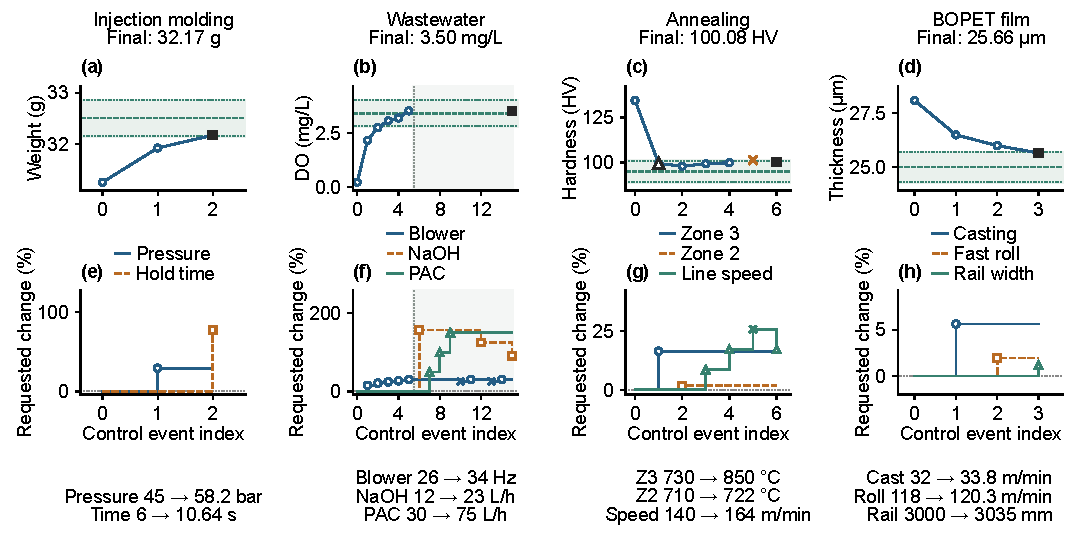
\includegraphics[width=\textwidth]{resources/fig-missions-controls.pdf}
\caption{Primary process-variable trajectories from the four-scenario
optimization campaign. The shaded band marks each target range, and the
horizontal axis orders scenario events. Circles show structured observations;
the open triangle marks the reverted annealing candidate, and open squares
mark mission-reported endpoints shown separately from structured observations.
The wastewater panel plots dissolved oxygen during aeration; later dosing and
cost-trimming actions address other variables.}
\label{fig:missions}
\end{figure*}

Injection molding and BOPET provide a contrast in actuator structure. Molding
uses paired hold adjustments to regulate one product measurement, whereas
BOPET distributes a thickness correction across three controls while retaining
its thermal operating range. The two missions therefore exercise the same
operation path with different signal maps and adjustment dimensions.

Annealing couples a production-rate objective to a product-quality constraint.
The controller increases line speed while checking hardness after each
candidate, and the route guard reverses the trial at the upper target boundary.
This sequence makes the quality constraint part of the decision process rather
than treating throughput as an independent setpoint objective.

Wastewater uses a staged process sequence. Aeration first brings dissolved
oxygen into its target range; chemical dosing then addresses pH and phosphorus
before the controller trims the modeled objective index. The ordered changes
show how one scenario can coordinate several process variables while retaining
an explicit relation between each intervention and its intended response.

Taken together, the four missions vary both actuator structure and objective
type, from product quality to throughput and a modeled process-cost index. The
blueprint supplies the scene-specific signals, targets, and guards; shared
dispatch, DCW execution, and DAQ observation carry the common operation
lifecycle. Table~\ref{tab:scenario-results} and Fig.~\ref{fig:missions} make
this relationship visible from configuration through outcome. The results
illustrate how application policies can change while the task-to-device
integration path remains consistent.
